% ============================================================
%  Knowledge-Based Systems (Elsevier) submission
%  Class: elsarticle  (the class KBS requires)
%  Compile: pdflatex -> bibtex -> pdflatex -> pdflatex
%           or simply:  ./build.sh
% ============================================================
\documentclass[review,12pt]{elsarticle}

\usepackage[T1]{fontenc}
\usepackage[utf8]{inputenc}
\usepackage{amsmath,amssymb}
\usepackage{graphicx}
\usepackage{booktabs}
\usepackage{tabularx}
\usepackage{array}
\usepackage{ragged2e}
\usepackage{enumitem}
\usepackage{caption}
\usepackage{lineno}
\usepackage{url}
\usepackage[hidelinks]{hyperref}

\captionsetup{font=small,labelfont=bf,justification=raggedright,singlelinecheck=false}
\setlist[itemize]{leftmargin=1.1em,itemsep=1pt,topsep=3pt,parsep=0pt}
\setlist[enumerate]{leftmargin=1.4em,itemsep=1pt,topsep=3pt,parsep=0pt}
\newcolumntype{L}[1]{>{\RaggedRight\arraybackslash}p{#1}}

% code identifiers are set in \texttt and cannot hyphenate; let them break
% after the underscore instead of running into the margin
\let\kgunderscore\_
\renewcommand{\_}{\kgunderscore\allowbreak}
\setlength{\emergencystretch}{2em}
\tolerance=400
\hbadness=10000

\graphicspath{{../figures/}}

\newcommand{\id}[1]{\texttt{#1}}

\journal{Knowledge-Based Systems}

\begin{document}

\begin{frontmatter}

\title{The Model Knows the Textbook but Not Your Class: Curriculum Knowledge
Graph Constraints for Slide Generation in Vocational Education}

% ---------------------------------------------------------------
% TODO(author): confirm the official English name of the institution.
%   The 2022 university charter gives "Jiangxi Ceramic Fine Arts Profession
%   Academy"; the current domain (jacti.edu.cn) and Xinhua (2025) use
%   "Jiangxi Arts & Ceramics Technology Institute". The latter is used here.
% ---------------------------------------------------------------
\author[a1]{Suxing Liu\corref{cor1}}
\ead{suxing.liu@example.edu.cn}
% \ead[url]{https://github.com/HAHA12345677888}

\affiliation[a1]{organization={School of Digital Media Technology, Jiangxi Arts
\& Ceramics Technology Institute},
  addressline={538 Xinchang West Road, Zhushan District},
  city={Jingdezhen},
  postcode={333001},
  state={Jiangxi},
  country={China}}

% TODO(author): enable if a second affiliation is required.
% \author[a2]{Suxing Liu}
% \affiliation[a2]{organization={School of Computer Sciences, Universiti Sains Malaysia},
%   city={Gelugor}, postcode={11800}, state={Penang}, country={Malaysia}}

\cortext[cor1]{Corresponding author.}

\begin{abstract}
Large language models can now produce a plausible-looking deck of lecture
slides in minutes, yet the output rarely survives a teacher's review: a skill
explicitly required by the syllabus is missing, the misconception that this
year's cohort keeps committing is repeated rather than corrected, or material
reserved for a later session is disclosed early. These failures are not defects
of generation capability. They arise because the relevant information is absent
from the model's parameters: course-level misconception inventories,
institution-specific sequencing decisions, and the code-level landing point of
a skill have never appeared in pretraining corpora.

We propose modelling such knowledge explicitly as a curriculum knowledge graph
and \emph{compiling} it, before generation, into an executable generation
contract that is subsequently used, after generation, as the acceptance
criterion. The central design decision is \emph{constraint-as-data}: the
contract is simultaneously the source of the prompt and the ground truth of the
validator, so that what is demanded and what is checked cannot drift apart. We
conduct a controlled study on the queue module of a higher-vocational
\emph{Python Data Structures} course (three sessions), covering six conditions
$\times$ three resamplings, three ablations, and a length-matched placebo arm:
78 independent generations in total.

The results differ from intuition, which is why they are worth recording.
Coverage rises from 0.61--0.70 at baseline to 0.98, and the length-matched
placebo demonstrates that this is not an artefact of longer prompts. Mean
misconception handling rises from 0.56 to 1.00, but the more informative change
is in dispersion: the standard deviation falls from 0.53 to 0.00. A condition
given the same misconception text without structure succeeds in roughly half of
its generations. What the graph changes is therefore not average quality but
\emph{reliability}. Ordering constraints, by contrast, show no reliable gain
under a strong model, and we do not defend that negative result. A blind review
by three teachers, who scored ten decks on five five-point items, reproduces the
automatic ordering: agreement over the overall score is ICC(2,3)~=~0.92, and the
rescaled misconception ratings track the automatic metric to within 0.09 on every
condition. We further document seven measurement defects discovered and corrected
during the study, each of which silently favours the constraint-based condition
and none of which raises an error---a general trap for text-level automatic
metrics in educational generation.
\end{abstract}

\begin{keyword}
curriculum knowledge graph \sep constrained generation \sep slide automation
\sep misconception modelling \sep educational knowledge engineering
\end{keyword}

% elsarticle flushes these into preliminary pages (before p.1) and resets the
% page counter after the highlights page, so the article opens on page 1.
% The graphical abstract is generated by paper/figures/make_graphical_abstract.py;
% the highlights are kept in step with highlights.tex (the standalone upload).
\begin{highlights}
  \item Course-level knowledge is absent from pretraining data; it must be supplied.
  \item A curriculum knowledge graph compiles into one contract that prompts and checks.
  \item Coverage rises from 0.61--0.70 to 0.98; a length-matched placebo rules out length.
  \item Misconceptions: 1.000 (0.000) vs 0.556 (0.527) when the text lacks structure.
  \item Order constraints give no reliable gain; seven metric defects are documented.
\end{highlights}

\begin{graphicalabstract}
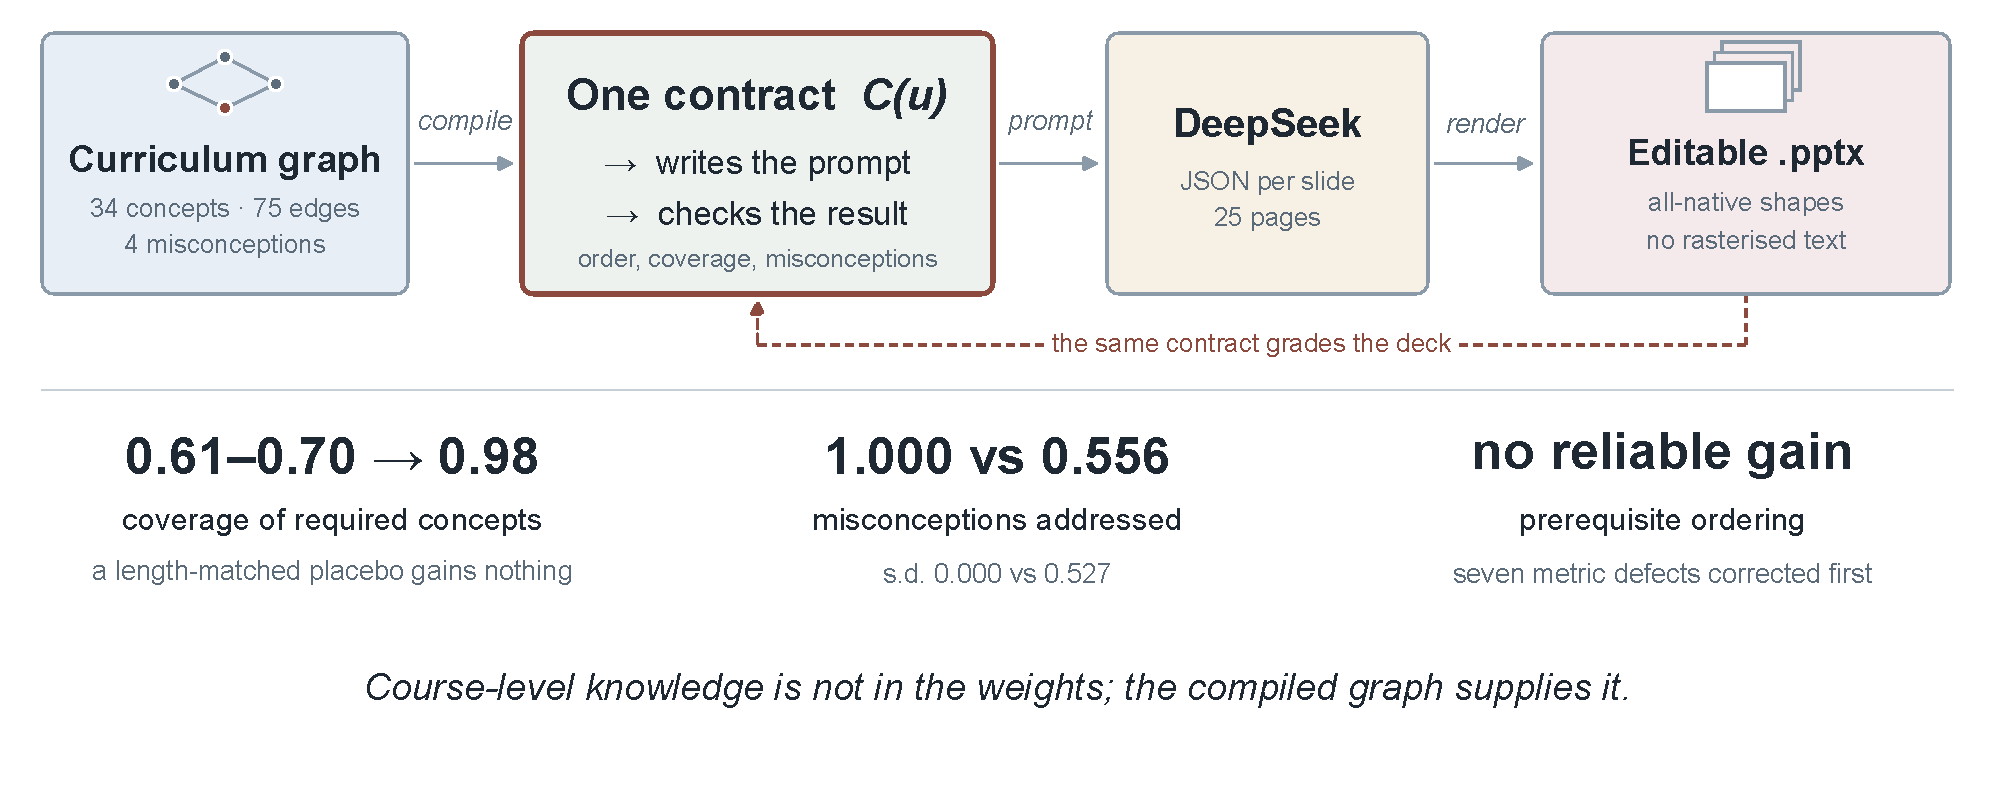
\includegraphics[width=\textwidth]{graphical_abstract.pdf}
\end{graphicalabstract}

\end{frontmatter}

\linenumbers

% ===============================================================
\section{Introduction}
% ===============================================================

\subsection{A concrete failure}

Asked to write the slides for a session on queues, a general-purpose large
language model (LLM) will typically return a well-organised deck with accurate
terminology and runnable code. A teacher skimming it will nod; a teacher reading
it closely will frown. The failures look like this.

\begin{itemize}
  \item The session objective states that students must \emph{implement}
  enqueue and dequeue on a sequential queue using a Python list. Across the six
  generated slides, however, the deck never shows \textbf{how to actually write
  it}. It covers the definition, covers the false-overflow problem, and covers
  the circular queue as the remedy---everything except the step the syllabus
  requires students to perform.
  \item The session carries a misconception that more than 60\% of this cohort
  reproduces in the final exam: ``a Python \id{list} is a linked list
  underneath.'' The model does not mention it, because it is not a textbook
  topic but a property of \emph{these} students.
  \item The model pushes the modular arithmetic of the circular queue into the
  slide on the sequential queue. Framed as ``broadening the view,'' it in fact
  violates the prerequisite order: students encounter \id{\% maxsize} before
  they know what \id{rear} is.
\end{itemize}

What these three failures share is that \textbf{none of them is a
generation-capability problem}. The model is perfectly able to write this
content. It simply does not know what \emph{this course} requires, where
\emph{this cohort} errs, and how \emph{this institution} sequences its sessions.

\subsection{Thesis}

We argue that the bottleneck in LLM-based slide generation has shifted from
\emph{knowledge acquisition} to the \textbf{representation and application of
course-level knowledge}. A general model possesses disciplinary knowledge (what
a queue is, why FIFO matters). Slide production requires \emph{situated}
knowledge: this course, this cohort, this schedule.

Situated knowledge has three properties, each of which happens to be a blind
spot of current LLMs (Table~\ref{tab:properties}).

\begin{table}[t]
\caption{Three properties of situated course knowledge and why they cannot be
acquired from pretraining.}
\label{tab:properties}
\footnotesize
\setlength{\tabcolsep}{5pt}
\begin{tabularx}{\linewidth}{@{}L{2.6cm}L{4.6cm}X@{}}
\toprule
Property & Example & Why the model cannot learn it \\
\midrule
Cohort-specific & This year's students confuse \emph{empty} and \emph{full}
conditions at a rate above 60\% &
Exists only in teacher experience and assignment statistics, in no public
corpus \\
Institution-specific & Our department merges ``linked queue'' and ``introducing
BFS'' into one session &
A teaching-office scheduling decision that varies by institution \\
Landing-point specific & This course requires ``can write the code,'' not merely
``can state the concept'' &
Set by the curriculum standard, not by the textbook \\
\bottomrule
\end{tabularx}
\end{table}

None of these can be obtained through a larger model or a better prompt; they
must be \textbf{supplied from outside}. The question then becomes: in what form
should they be supplied, such that the model can follow them \emph{and} the
system can afterwards check whether it did?

\subsection{Our answer}

A \textbf{knowledge graph}. The justification is not fashion but the fact that
it satisfies four requirements at once.

\begin{enumerate}
  \item \textbf{Expressiveness.} Misconceptions, skills, prerequisite relations,
  and competence levels are heterogeneous entities; a graph accommodates them
  naturally.
  \item \textbf{Orderability.} \id{prerequisites\_for} is a directed edge, so a
  topological sort directly yields a legal teaching order.
  \item \textbf{Compilability.} The subgraph of one session can be mechanically
  compiled into a generation contract (concept inventory, order, misconceptions,
  forbidden terms).
  \item \textbf{Reusability as ground truth.} The same contract can be used to
  validate the output---\textbf{what is demanded and what is checked share one
  source, and cannot drift}.
\end{enumerate}

Point~4 is the essential difference from ``writing the key points into the
prompt.'' A prompt is discarded once written, and there is no way afterwards to
determine whether the model complied. A contract is a data object, readable by
programs both before and after generation.

\subsection{Contributions}

\begin{enumerate}
  \item \textbf{A curriculum-graph schema for vocational programming courses.}
  We extend the seven node types of K12-KGraph~\cite{liang2026k12kgraph} by
  promoting \id{Misconception} to a first-class node, and add two edge types:
  \id{implements} (concept $\to$ executable code) and
  \id{addresses\_misconception} (teaching unit $\to$ misconception). The former
  makes ``can write it'' a checkable property; the latter makes corrective
  content a constrainable generation target.

  \item \textbf{A constraint-as-data generation framework.} \id{UnitConstraints}
  drives both prompt construction and post-hoc validation; topological order,
  required/optional partitioning, sibling-session background caps, and
  forbidden-term lists are all derived mechanically from the subgraph, with no
  hand-written rules.

  \item \textbf{A reproducible six-metric acceptance protocol}, two of whose
  metrics are redefined for this task: prerequisite order is judged by
  \emph{where a concept is named in a slide title} (not by model-reported IDs),
  and coverage is matched against \emph{graph synonyms} (so that a condition
  copying the source wording gains no advantage).

  \item \textbf{An honest empirical study.} Six conditions $\times$ three
  sessions $\times$ three resamplings, plus three ablations and a length-matched
  placebo: 78 independent generations. We report gains \emph{and} the absence of
  gain: misconception handling differs decisively in both mean and variance;
  coverage improves by about 0.3 with the length explanation excluded by the
  placebo; and ordering constraints show no reliable contribution under a strong
  model. We also document \textbf{seven} measurement defects that systematically
  favour constraint-based methods, together with their fixes (\S\ref{sec:defects}).

  \item \textbf{A blind teacher review that independently reproduces the automatic
  ordering.} Three teachers scored ten decks on five five-point items and an
  overall score, yielding ICC(2,3)~=~0.92 for the overall rating. Rescaled to
  $[0,1]$, their misconception ratings fall within 0.09 of the automatic metric on
  all four conditions, and they place the difference between conditions on the
  same axis: misconception handling and coverage, not factual accuracy.
\end{enumerate}

\subsection{Why this belongs in \emph{Knowledge-Based Systems}}

The object of this paper is not ``a better slide generator'' but \textbf{how
knowledge must be represented in order to be actionable by a machine}: what
structure suffices to constrain generation, how it is compiled, how it is
verified, and along which dimensions a knowledge base is genuinely
irreplaceable. This matches the knowledge-representation, reasoning and
system-evaluation loop that this journal serves.

Three recent contributions in this journal form the immediate context. Dai et
al.~\cite{dai2025kg} systematically compare how LLMs comprehend knowledge graphs
presented in different prompt formats (linearised triples, fluent natural
language, neighbourhood expansion), showing that \textbf{the presentation format
itself changes performance}. Huang et al.~\cite{huang2025longtail} find that
graph-triple prompting generally outperforms passage prompting on long-tail
factual question answering, and that combining them markedly reduces
hallucination, showing that \textbf{structure and text are not interchangeable}.
Ma et al.~\cite{ma2026ledlcm} apply knowledge-enhanced LLMs to course
recommendation, placing education among the journal's active application areas.
We continue this line but move the question from \emph{how to put knowledge in}
to \emph{whether the knowledge once inserted can also serve as the acceptance
criterion}.

We emphasise \textbf{negative results}: a knowledge graph is not superior to a
strong model along every dimension, and identifying \emph{which} knowledge must
be externalised is more valuable than a blanket claim that knowledge
augmentation works.

% ===============================================================
\section{Related work}
% ===============================================================

\subsection{Automatic slide generation}

Three strands can be distinguished, each solving a different problem.

\paragraph{Document-to-slide: fidelity to the input}
DOC2PPT~\cite{fu2022doc2ppt} first formalised the task, observing that it
simultaneously demands document summarisation, figure--text retrieval and layout
arrangement. It proposed a hierarchical sequence-to-sequence model and released
5{,}873 paired document--slide examples drawn from computer-vision, ACL and ICML
proceedings, together with four metrics (slide-level ROUGE, LC-FS, TFR, mIoU).
Mondal et al.~\cite{mondal2024presentations} introduced \emph{end-user
specifications}: the same paper should yield different decks for different
audiences or durations. They built four persona configurations on SciDuet,
fine-tuned an LLM on target-audience feedback, and cut preparation time from
about one hour to under thirty minutes. Notably, the authors state in their
limitations that they \textbf{do not address slide layout design}; the
contribution is content and logical alignment only.

\paragraph{Instruction-to-slide: fidelity to editability}
AutoPresent~\cite{ge2025autopresent} released SlidesBench (7k training and 585
test examples from 310 real decks across ten domains) and compared end-to-end
image generation against program generation, concluding that
\textbf{programmatic generation yields higher-quality slides} because the
artefacts are interactive and re-editable; an 8B model trained on the benchmark
matches GPT-4o. PPTAgent~\cite{zheng2025pptagent} adopts a two-stage edit-based
approach: analyse reference decks to extract slide-level functional types and
content schemas, then draft an outline and iteratively generate editing actions,
with PPTEval assessing content, design and coherence. Our rendering decisions
(native shapes, a mandatory JSON intermediate representation) follow this
strand's conclusions.

\paragraph{Evaluation: from ``does it look right'' to ``is it done''}
PPTC~\cite{guo2024pptc} changes the question from whether slides look good to
whether a model can modify a deck correctly under multi-turn instructions. Its
279 multi-turn sessions come with PPTX-Match, which compares the resulting
\id{.pptx} file state rather than the API sequence and therefore admits multiple
valid solutions. GPT-4 reaches 75.1\% single-turn accuracy but only 6\% session
accuracy, with errors traced to multi-turn accumulation, long template
processing and multimodal perception.

\paragraph{Our difference}
The inputs to the above work are a \emph{document to be compressed} or \emph{a
single instruction}; the criteria are resemblance to the source, visual appeal,
or task completion. Our input is a \emph{course specification} (what to teach,
in what order, which misconception to correct, what not to introduce), and the
criterion is conformance to the syllabus. This is not a relabelling: neither the
reference-based nor the reference-free protocol of SlidesBench can express ``the
deck omits the skill the syllabus requires students to implement,'' which is
precisely the most damaging class of failure in a teaching context.

\subsection{Educational knowledge graphs}

K12-KGraph~\cite{liang2026k12kgraph} is the closest knowledge-side work.
Extracted from the official People's Education Press textbooks, it defines seven
node types (Book, Chapter, Section, Concept, Skill, Experiment, Exercise) and
nine relation types (\id{is\_a}, \id{prerequisites\_for}, \id{relates\_to},
\id{verifies}, \id{tests\_concept}, \id{tests\_skill}, \id{appears\_in},
\id{leads\_to}, \id{is\_part\_of}), covers 48 volumes across mathematics,
physics, chemistry and biology, and yields 10{,}685 nodes and 23{,}278 edges.
From it the authors derive K12-Bench (23{,}640 multiple-choice items in five task
families: Ground, Prereq, Neighbor, Evidence, Locate) and K12-Train, a
graph-guided supervised fine-tuning corpus. Its most telling number is not the
overall score but the fact that \textbf{even the strongest proprietary model
leaves more than 40\% of Prereq and Neighbor items unsolved}---evidence that
structural curriculum cognition is a capability dimension independent of factual
recall, and precisely the dimension we attempt to supply externally.

SciMKG~\cite{lu2026scimkg} moves to multimodality: an LLM-driven
extraction--verification--integration--augmentation pipeline builds a graph over
text, images, video and audio from open courseware, yielding 1{,}356 knowledge
points, 34{,}630 multimodal concepts and 403{,}400 triples, with
concept-extraction F1 improved by 9\% over baselines. On the application side,
Ma et al.~\cite{ma2026ledlcm} apply knowledge-enhanced LLMs to course
recommendation, confirming sustained interest in the combination of knowledge
structure and education.

The centre of gravity in this literature is \emph{building} graphs (extracting
entities and relations from corpora, ensuring consistency). Ours is \emph{using}
them (compiling a graph into generation constraints and validating against it).
The two are complementary: our method can consume graphs produced by the above
work directly, and indeed we reuse the K12-KGraph node and relation skeleton,
adding to it rather than replacing it (\S\ref{sec:construction}).

In vocational education, a graph must additionally express two things that
general subject-matter graphs do not emphasise: \textbf{competence level}
(understand, comprehend, master, proficient, which decides whether a concept is
mandatory or optional) and \textbf{typical misconceptions} (which decide
corrective content). K12-KGraph carries an \id{importance} attribute on concepts
but does not use it to constrain generation; misconceptions are absent entirely.
This is the direct motivation for our schema extension.

\subsection{Constrained generation}

Classical natural language generation separates \emph{what to say and in what
order} (content planning) from \emph{how to say it} (surface
realisation)~\cite{gatt2018survey}. Wiseman et al.~\cite{wiseman2017challenges}
showed on RotoWire that end-to-end models produce fluent game reports while
systematically erring on content selection and discourse order, in some metrics
even being surpassed by template baselines. Puduppully et
al.~\cite{puduppully2019datatotext} therefore model content planning explicitly:
first predict which records to mention and in what order, then generate
conditioned on that plan. What unites this line is that structure is injected
into the \emph{training objective or the decoding process}.

In the LLM era, structure is injected through prompts instead, and the question
becomes \emph{in what form}. Dai et al.~\cite{dai2025kg} provide the most
systematic evidence to date: the same graph, presented as linearised triples,
fluent paragraphs or expanded neighbourhoods, is comprehended with markedly
different effectiveness, and the difference is explicable from attention
distributions. Huang et al.~\cite{huang2025longtail} offer a complementary
result on long-tail factual question answering: triple-based prompting generally
beats passage-based prompting, and combining both does not always improve
coverage but does markedly reduce hallucination. In short, \textbf{structured
knowledge is not simply ``text written differently.''}

We differ from both lines deliberately: we neither train, nor modify decoding,
nor rerank. We compile constraints into an \emph{executable data object}, use it
to construct the prompt before generation, and use the same object to validate
afterwards. Relative to~\cite{dai2025kg,huang2025longtail}, the question
advances from ``how should a graph enter the prompt'' to ``can one graph
simultaneously serve as the acceptance criterion''---if so, demand and check
cannot drift (\S 1.3). The price is that we relinquish control over decoding and
must bear the risk that the model disobeys; \S\ref{sec:qualitative} reports a
real violation and \S\ref{sec:defects} reports seven metric traps that this
permissiveness exposed.

% ===============================================================
\section{Problem formulation}
% ===============================================================

\subsection{Curriculum knowledge graph}

A curriculum knowledge graph is a typed directed heterogeneous graph
$G=(V,E,\tau)$, where $\tau: V \to T_V$ with
\begin{equation*}
T_V=\{\text{Course},\text{Module},\text{Unit},\text{Concept},\text{Skill},
\text{Lab},\text{Exercise},\text{Misconception}\};
\end{equation*}
each edge $e=(u,r,v)\in E$ carries a relation type $r\in T_E$ with
\begin{align*}
T_E=\{&\text{is\_a},\ \text{prerequisites\_for},\ \text{relates\_to},\
\text{implements},\\
&\text{verified\_by},\ \text{assessed\_by},\
\text{addresses\_misconception},\\
&\text{appears\_in},\ \text{is\_part\_of},\ \text{leads\_to}\};
\end{align*}
and selected edges carry an \id{evidence} field recording the provenance of the
relation (textbook page, curriculum-standard clause, error-rate statistic).

\paragraph{Constraint 1 (acyclicity)} The subgraph induced by
\id{prerequisites\_for} must be a DAG. We detect violations with Kahn's
algorithm: if the concept set of a session cannot be topologically ordered, the
course design itself contains a circular prerequisite, and construction fails
immediately rather than deferring the contradiction to generation time.

\subsection{Session contract}

For a session $u\in V$ with $\tau(u)=\text{Unit}$, take the subgraph
\begin{equation}
G_u = \{\,v \in V : (v,\text{appears\_in},u)\in E\,\}
\end{equation}
and compile it into a contract
\begin{equation}
C(u)=\langle S_u,\ \prec_u,\ M_u,\ F_u,\ B_u,\ k_u\rangle ,
\end{equation}
whose components are given in Table~\ref{tab:contract}.

\begin{table}[t]
\caption{Components of the session contract $C(u)$ and where each is read from
in the graph.}
\label{tab:contract}
\footnotesize
\setlength{\tabcolsep}{5pt}
\begin{tabularx}{\linewidth}{@{}L{1.6cm}L{5.4cm}X@{}}
\toprule
Symbol & Meaning & Source \\
\midrule
$S_u=(R_u,O_u)$ & required / optional concept sets &
split on \id{importance}; at or above ``master'' is required \\
$\prec_u$ & teaching order (a total order on $S_u$) &
topological order of \id{prerequisites\_for} over $G_u$ \\
$M_u$ & misconceptions that must be corrected &
\id{Misconception} nodes targeted by \id{addresses\_misconception} \\
$F_u$ & forbidden-term list & \id{forbidden\_terms} on the Unit node \\
$B_u$ & sibling-session concepts admissible as brief recap &
concepts of other Units in the same Module, deduplicated \\
$k_u$ & slide budget & \id{slide\_budget} on the Unit node \\
\bottomrule
\end{tabularx}
\end{table}

A critical distinction separates $B_u$ from $F_u$. The former means ``already
covered, may be mentioned in one sentence''; the latter means ``not taught in
this course at all.'' Conflating them makes two metrics fight each other (the
same term counts both as legitimate recap and as out-of-scope), so the
implementation enforces mutual exclusivity by assertion.

Compilation is mechanical and lossless. Fig.~\ref{fig:contract} shows the actual
U11 subgraph and the contract compiled from it: every edge in panel~(a) maps to a
field in panel~(b), and nothing in panel~(b) is hand-written.

\subsection{Generation and acceptance}

Generation is a mapping $D = f_\theta(C(u))$ where $D$ is a sequence of slides.
Acceptance is a metric vector
\begin{equation}
m(D, C(u), G) = \langle \text{cov},\ \text{oog},\ \text{bg},\
\text{pre},\ \text{mc},\ \text{edit}\rangle
\end{equation}
defined in \S\ref{sec:metrics}. Note that $C(u)$ appears on both sides: this is
the formal statement of ``demand and check share one source.''

The full pipeline is shown in Fig.~\ref{fig:framework}: graph $\to$ contract
compilation $\to$ generation $\to$ rendering $\to$ validation against the same
contract. One loop exists: pages that fail validation are sent back for
regeneration. Its boundary is deliberately fixed---\textbf{the loop may change
slides, but never the graph and never the contract}---and whether to regenerate
is a teacher's decision, not an automatic optimisation. Were validation output
allowed to reshape the contract, acceptance would degrade into an objective and
the metrics would lose their meaning (\S\ref{sec:defects}).

\begin{figure}[t]
\centering
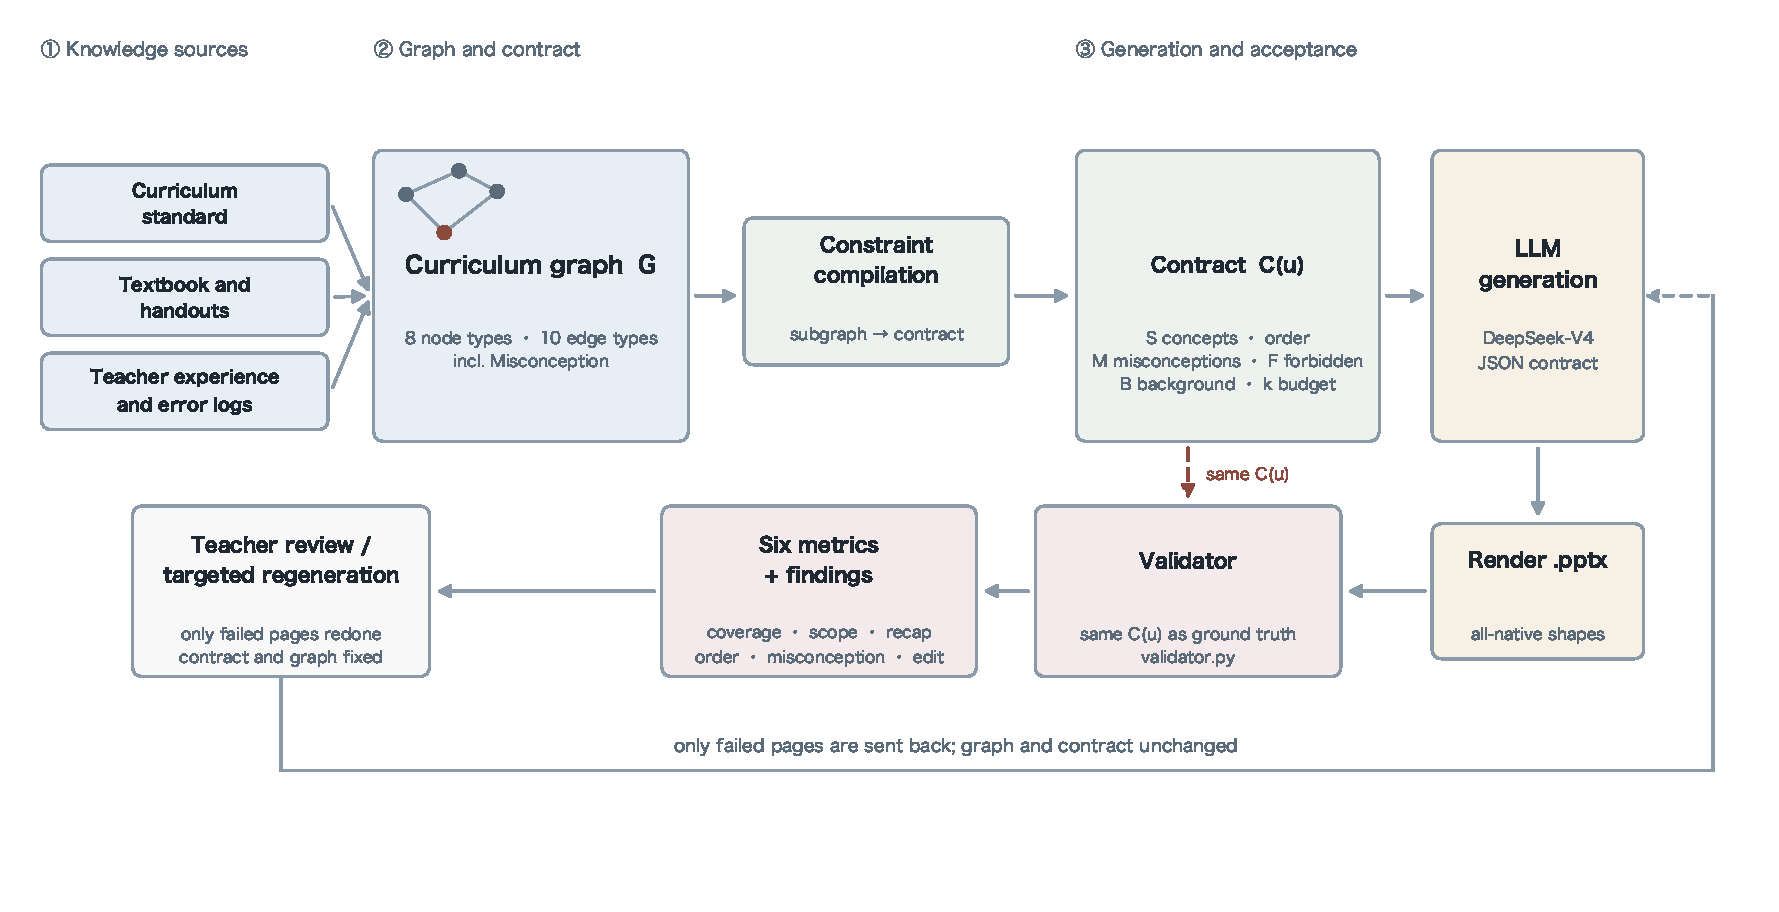
\includegraphics[width=\linewidth]{framework_en.pdf}
\caption{Framework overview. The contract $C(u)$ is read once before generation
(to build the prompt) and once after (to compute the six metrics); both reads
concern the same object, which is what ``demand and check share one source''
means in implementation terms.}
\label{fig:framework}
\end{figure}

\begin{figure}[t]
\centering
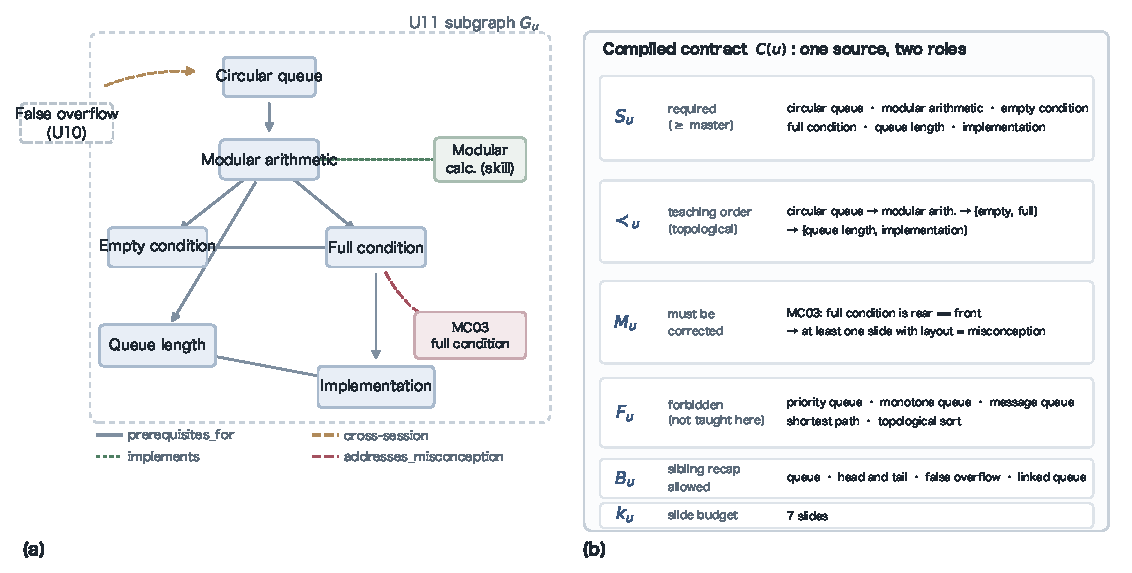
\includegraphics[width=\linewidth]{graph_contract_en.pdf}
\caption{From subgraph to contract. (a) The actual U11 subgraph in the released
graph file: six concepts and one skill, seven intra-session prerequisite edges,
one cross-session prerequisite edge from U10, one \id{implements} edge and one
\id{addresses\_misconception} edge. (b) The contract $C(u)$ produced from it by
\id{build\_constraints}; the validator subsequently reads the same object.}
\label{fig:contract}
\end{figure}

% ===============================================================
\section{Method}
% ===============================================================

\subsection{Graph construction}
\label{sec:construction}

\subsubsection{Nodes and edges}

We retain the seven node types of K12-KGraph~\cite{liang2026k12kgraph} (\id{Lab}
corresponds to its \id{Experiment}) and promote \id{Misconception} to an eighth,
with attributes \id{statement} (the erroneous claim itself, which must be
concrete and decidable), \id{correction}, \id{frequency} (low, common, high) and
\id{evidence} (exam error rate, assignment statistics, in-class questioning).

Two edge types are added:
\begin{itemize}
  \item \id{implements}: Concept or Skill $\to$ executable code fragment. It makes
  ``can write it'' a checkable property and supplies the generator with runnable
  examples.
  \item \id{addresses\_misconception}: Unit, Lab or Concept $\to$ Misconception,
  annotated with a strategy (counter-example, code demonstration, boundary test).
  This edge decides \textbf{which session is responsible} for correcting a given
  misconception, preventing both duplication across sessions and orphaned
  misconceptions.
\end{itemize}

\subsubsection{Synonyms}

Every concept may carry aliases. This is not a patch for evaluation but
legitimate graph content: in class the teacher says ``judging full,'' the
textbook writes ``the full condition,'' and the code reads
\id{(rear+1) \% maxsize == front}; all three denote one entity. Without aliases
the graph cannot be aligned with real teaching language. Aliases also resolve a
fairness problem in evaluation, as discussed in \S\ref{sec:defects}.

\subsection{Constraint compilation}

\id{build\_constraints} turns the subgraph into a \id{UnitConstraints} object
with no hand-written rules:
\begin{enumerate}
  \item \textbf{Required/optional split.} Sort by \id{importance}; those at or
  above ``master'' enter $R_u$, the rest $O_u$.
  \item \textbf{Topological order.} Run Kahn's algorithm over $S_u$; on
  encountering a cycle, fall back to declaration order and raise a warning.
  \item \textbf{Misconception assignment.} Collect the misconception nodes
  attached by \id{addresses\_misconception} edges.
  \item \textbf{Sibling sessions.} Concept names of other Units in the same
  Module, minus those already in this session.
  \item \textbf{Evidence anchors.} Collect \id{evidence} along incoming
  \id{prerequisites\_for}, \id{implements} and \id{verified\_by} edges, and
  render them as \emph{teacher-facing} verification material, explicitly
  labelled ``not generated content'' so that the model does not copy the
  provenance into the slides as body text.
\end{enumerate}

The compilation output is a \emph{deterministic string}: the same graph always
yields the same prompt block, which is a precondition for reproducibility.

\subsection{Generation}

The prompt is assembled from four segments---a fixed skeleton, the contract
block, a JSON contract, and a list of hard rules---and the experimental
conditions of \S\ref{sec:conditions} replace only some of them.

Output is constrained to a single JSON object, each slide carrying \id{layout}
(one of seven), \id{title}, \id{bullets}, \id{code}, \id{notes},
\id{concept\_ids} and \id{background}. Forcing JSON rather than free-form layout
is a deliberate choice: layout selection is itself an instructional-design
decision, and delegating it to the model makes both editability and slide budget
uncontrollable.

Two engineering realities, both observed rather than assumed:
\begin{enumerate}
  \item \textbf{JSON mode is not a validity guarantee.} Roughly once every ten
  calls the response contains a trailing comma, or returns blank while reporting
  \id{finish\_reason == "stop"} (the offending fragment replaced by whitespace).
  The pipeline therefore implements \emph{call} $\to$ \emph{conservative repair}
  (strip trailing commas, close truncated brackets) $\to$ \emph{parse}, and only
  escalates by re-prompting with the concrete parse error when repair fails.
  Blind retries reproduce the same error at the same cost.
  \item \textbf{The model performs internal reasoning by default.} Every call in
  our setup produced \id{reasoning\_tokens}, which contaminates a
  chain-of-thought baseline (the model is already doing CoT). We record the
  setting explicitly and provide a switch to disable it for a robustness check.
\end{enumerate}

\subsection{Rendering}

\id{python-pptx} emits 16:9 fully native shapes with no rasterised text.
\id{editability} is defined as the ratio of native editable shapes to all shapes;
it is 1.0 for every condition here. This dimension does not discriminate between
methods; it exists to exclude ``screenshot-style generation,'' whose value for a
teacher who needs to edit is zero.

For Chinese text, the East-Asian and complex-script typeface attributes must be
set explicitly, otherwise presentation software falls back to a Latin font and
glyphs are corrupted.

\subsection{Validation}

The six metrics are defined in \S\ref{sec:metrics}. Three implementation choices
are deliberate.

\begin{itemize}
  \item \textbf{Chinese has no word boundaries.} The term for \emph{queue} matches
  inside the term for \emph{circular queue}. All counting therefore uses per-line
  net occurrences: raw count minus occurrences covered by longer terms
  \emph{within the same line}. Subtracting over the whole document rather than
  per line is a real bug: an independent occurrence on slide~2 is otherwise
  cancelled by a compound term on slide~4.
  \item \textbf{Triple-criterion misconception detection.} Structural anchor
  (does the misconception slide reference a graph-linked concept), then
  English-identifier overlap (\id{rear}, \id{list}), then Chinese character
  bigram overlap (threshold 0.35). Purely lexical matching misses cases where
  the model paraphrases the erroneous claim in its own words; we observed a
  generated correction slide rejected because its phrasing differed from the
  graph's.
  \item \textbf{Order by first textual position}, see \S\ref{sec:metrics}.
\end{itemize}

% ===============================================================
\section{Experiments}
% ===============================================================

\subsection{Course and data}

The target course is \emph{Python Data Structures}, a higher-vocational
programme in Artificial Intelligence Technology Application with 136 contact
hours. The graph scope is Module M4, ``Queues'', comprising three sessions (U10,
concepts and false overflow; U11, circular queue; U12, linked queue and
introducing breadth-first search), with 34 nodes, 75 edges and four
misconceptions. The prerequisite chain in this module is clean (queue $\to$
sequential queue $\to$ circular queue $\to$ linked queue), whereas
deep-learning courses have mutually referencing concepts that easily form
cycles and are therefore unsuitable as a first validation scenario.

The goal is to establish \emph{whether and along which dimensions} graph
constraints help, not to maximise a course-wide number. Three sessions cover
three qualitatively different cases: concept-dense (U11 has seven required
concepts), skill-landing (U10 contains a skill that must be implemented by hand),
and application-introduction (U12 requires a comparative selection against prior
material).

\subsection{Conditions}
\label{sec:conditions}

Six conditions carry strictly increasing information, each step removing one
structural element (Table~\ref{tab:conditions}).

\begin{table}[t]
\caption{Six experimental conditions. Prompt lengths are measured on session
U11, in characters.}
\label{tab:conditions}
\footnotesize
\setlength{\tabcolsep}{4pt}
\begin{tabularx}{\linewidth}{@{}L{1.5cm}cccccc@{}}
\toprule
Condition & Course/ & Page & Concept names & Topological & Misconceptions & Forbidden
\\
 & session & budget & + definitions & order & & terms \\
\midrule
\id{full} (ours) & \checkmark & \checkmark & \checkmark & \checkmark &
\checkmark & \checkmark \\
\id{rag\_mc} & \checkmark & \checkmark & \checkmark & -- & \checkmark & -- \\
\id{rag} & \checkmark & \checkmark & \checkmark & -- & -- & -- \\
\id{placebo} & \checkmark & \checkmark & -- & -- & -- & -- \\
\id{cot} & \checkmark & \checkmark & -- & -- & -- & -- \\
\id{zero\_shot} & \checkmark & \checkmark & -- & -- & -- & -- \\
\midrule
Prompt length (U11) & \multicolumn{6}{r}{1997 / 1122 / 997 / 2195 / 625 / 585} \\
\bottomrule
\end{tabularx}
\end{table}

\begin{itemize}
  \item \id{rag} $-$ \id{zero\_shot} measures the contribution of \emph{content
  retrieval}.
  \item \id{full} $-$ \id{rag} measures the contribution of \emph{structural
  constraints}.
  \item \id{rag\_mc} is a control built specifically for the misconception claim:
  the same misconception text is supplied as a flat passage, but without
  ordering and without layout requirements. If \id{full} still wins on the
  misconception metric, the gain comes from \emph{structuring the text to the
  point where it constrains layout}, not from \emph{the text appearing in the
  prompt}.
  \item \id{placebo} is a control built specifically for the alternative
  explanation ``the prompt is simply longer'': the prompt is
  \emph{length-matched} to \id{full} (in fact slightly longer), but padded with
  generic slide-writing advice unrelated to this course. If the advantage of
  \id{full} were prompt length, the placebo should catch up. It does not
  (\S\ref{sec:results}).
\end{itemize}

Three ablations retain the complete contract and rule wording of \id{full},
deleting exactly one data block (Table~\ref{tab:ablations}).

\begin{table}[t]
\caption{Three ablations. The corresponding rule text is removed together with
the data block.}
\label{tab:ablations}
\footnotesize
\setlength{\tabcolsep}{5pt}
\begin{tabularx}{\linewidth}{@{}L{3.2cm}L{2.7cm}L{1.7cm}X@{}}
\toprule
Condition & Removed & Rule also removed & Expected metric \\
\midrule
\id{no\_order} & order block & rule 3 & \id{prerequisite\_violation} \\
\id{no\_misconception} & misconception block & rule 5 & \id{misconception\_coverage} \\
\id{no\_forbidden} & forbidden-term block & rule 6 & \id{oog\_rate} \\
\bottomrule
\end{tabularx}
\end{table}

The rule text must be removed together with the data. Deleting only the data
while keeping a rule that says ``you must follow the given order'' forces the
model to guess an order, and the ablation is no longer clean; a unit test guards
this.

\subsection{Metric definitions}
\label{sec:metrics}

The six metrics are listed in Table~\ref{tab:metrics}.

\begin{table}[t]
\caption{Metric definitions. Arrows indicate the desired direction.}
\label{tab:metrics}
\footnotesize
\setlength{\tabcolsep}{5pt}
\begin{tabularx}{\linewidth}{@{}L{4.0cm}Xc@{}}
\toprule
Metric & Definition & Direction \\
\midrule
\id{coverage\_rate} & fraction of required concepts actually taught & $\uparrow$ \\
\id{oog\_rate} & (out-of-graph IDs + forbidden-term hits) / (covered + out-of-graph) & $\downarrow$ \\
\id{background\_rate} & characters devoted to sibling-session concepts / total characters (cap 25\%) & $\downarrow$ \\
\id{prerequisite\_violation} & violated concept pairs / all concept pairs & $\downarrow$ \\
\id{misconception\_coverage} & misconceptions corrected / misconceptions linked to the session & $\uparrow$ \\
\id{editability} & native editable shapes / all shapes & $\uparrow$ \\
\bottomrule
\end{tabularx}
\end{table}

Three definitional decisions determine the conclusions and therefore require
explicit justification:
\begin{enumerate}
  \item \textbf{Coverage counts body slides only.} Title, objectives and summary
  slides list every concept by definition; counting them as ``taught'' lets a
  deck consisting of a table of contents score full marks.
  \item \textbf{Coverage matches on name and aliases.} Otherwise the \id{full}
  condition, which copies source names, enjoys a structural advantage
  (\S\ref{sec:defects}).
  \item \textbf{Order is judged by first textual position.} The model's
  \id{concept\_ids} are self-reported, and the three baselines were never told the
  field exists. Scoring on self-reports means a completely empty answer receives
  a zero violation rate.
\end{enumerate}

\subsection{Results}
\label{sec:results}

Each condition runs three sessions $\times$ three resamplings, that is, nine
independent generations; each ablation runs six. Values are mean (standard
deviation).

\begin{table}[t]
\caption{Main results ($n=9$), mean (standard deviation). Cov.: coverage; OOG:
out-of-graph; Bg.: background; Ord.: prerequisite violation; Miscon.:
misconception. Best value per column in bold. Editability is 1.000 for every
condition and is therefore omitted.}
\label{tab:main}
\scriptsize
\setlength{\tabcolsep}{3pt}
\begin{tabularx}{\linewidth}{@{}L{2.55cm}cccccc@{}}
\toprule
Condition & Cov. $\uparrow$ & OOG $\downarrow$ & Bg. $\downarrow$
& Ord. $\downarrow$ & Miscon. $\uparrow$ & Pass rate \\
\midrule
\textbf{\id{full} (ours)} & \textbf{0.981} (0.056) & \textbf{0.000} & 0.027 (0.016)
& \textbf{0.020} (0.045) & \textbf{1.000} (0.000) & 67\% \\
\id{rag\_mc} & 0.698 (0.295) & 0.111 (0.220) & 0.027 (0.016) & 0.007 (0.022)
& 0.556 (0.527) & 22\% \\
\id{rag} & 0.659 (0.248) & 0.111 (0.220) & 0.032 (0.014) & 0.030 (0.089)
& 0.222 (0.441) & 0\% \\
\id{placebo} & 0.675 (0.266) & 0.167 (0.250) & 0.040 (0.018) & 0.096 (0.131)
& 0.333 (0.500) & 0\% \\
\id{cot} & 0.614 (0.185) & 0.019 (0.056) & 0.040 (0.016) & 0.089 (0.183)
& 0.389 (0.486) & 0\% \\
\id{zero\_shot} & 0.643 (0.248) & 0.019 (0.056) & 0.040 (0.011) & 0.037 (0.089)
& 0.222 (0.441) & 0\% \\
\bottomrule
\end{tabularx}
\end{table}

Four observations follow, ordered by importance.

\paragraph{(1) Coverage: 0.981 against 0.61--0.70, and not an effect of prompt
length} The five controls lie within 0.09 of one another (0.614--0.698) while
all have large dispersion (0.19--0.30); \id{full} is about 0.3 higher with
dispersion down to 0.056. The decisive evidence is the placebo: its prompt is
comparable in length to \id{full} (2195 against 1997 characters on U11, in fact
longer), but its content is generic writing advice unrelated to the course, and
its coverage is 0.675, indistinguishable from zero-shot. The coverage gain
therefore comes from \textbf{course structure}, not from saying more.

\paragraph{(2) Misconception: the mean is the lesser finding; the disappearance
of variance is the greater} This is the strongest evidence in the paper.
\id{rag\_mc} gives the model the same misconception text and reaches a mean of
0.556, but with a standard deviation of 0.527: it succeeds reliably in only about
half of nine generations. \id{full} reaches 1.000 with zero dispersion. In other
words, \textbf{telling the model the knowledge yields a system that depends on
luck; structuring the knowledge into a layout requirement yields a reliable
system.} This is precisely our thesis: the value of the graph is not that it
conveys content but that it forces content to appear \emph{at a specific
position}.

\paragraph{(3) Ordering: the constraint helps but not significantly, and adds no
reliable marginal contribution} The violation rate of \id{full} (0.020) is below
that of the placebo (0.096) and \id{cot} (0.089), but \id{zero\_shot} sits at
0.037: a condition given no ordering information at all is nearly as good. This
is consistent with the ablation below and with the explanation that strong models
already have a sound intuition for textbook prerequisite chains. We do not defend
it: \textbf{on this task, ordering is not where the knowledge graph earns its
keep.}

\paragraph{(4) Out-of-graph: \id{rag} and \id{rag\_mc} are worse than
zero-shot} Both reach an out-of-graph rate of 0.111 and the placebo 0.167,
whereas \id{zero\_shot} sits at 0.019 and \id{full} at 0. Telling the model
``this session covers these points'' leads it to bring in adjacent advanced
material (mentioning priority queues in a session on queues), because the prompt
demarcates a scope without demarcating a boundary. \id{full} reaches zero only by
virtue of the forbidden-term list, an explicit negative example, as the ablation
confirms.

\begin{table}[t]
\caption{Ablations; each removes exactly one part of the graph ($n=6$).}
\label{tab:ablation}
\footnotesize
\setlength{\tabcolsep}{5pt}
\begin{tabularx}{\linewidth}{@{}L{3.2cm}cccc@{}}
\toprule
Condition & Coverage $\uparrow$ & Out-of-graph $\downarrow$ & Order viol. $\downarrow$
& Misconception $\uparrow$ \\
\midrule
\id{full} & 1.000 (0.000) & 0.000 (0.000) & 0.032 (0.078) & 1.000 (0.000) \\
$-$ ordering & 1.000 (0.000) & 0.000 (0.000) & 0.000 (0.000) & 1.000 (0.000) \\
$-$ misconceptions & 0.944 (0.086) & 0.000 (0.000) & 0.040 (0.064)
& \textbf{0.167} (0.408) \\
$-$ forbidden terms & 1.000 (0.000) & \textbf{0.083} (0.129) & 0.000 (0.000)
& 1.000 (0.000) \\
\bottomrule
\end{tabularx}
\end{table}

The ablation (Table~\ref{tab:ablation}) yields two positives and one negative,
cleanly separated:
\begin{itemize}
  \item Removing the misconception block drops misconception coverage from 1.000
  to 0.167 and coverage from 1.000 to 0.944; the block carries corrective content
  and incidentally helps the model organise the session's key points.
  \item Removing the forbidden-term list raises the out-of-graph rate from 0.000
  to 0.083 with every other metric unchanged: single responsibility, clean
  attribution.
  \item Removing the ordering constraint drops the violation rate from 0.032 to
  \textbf{0.000}, opposite to expectation. This is not a measurement error:
  \id{full}'s 0.032 traces to one genuine inversion in U10 (sequential queue
  taught before head and tail). At the scale of seven concepts and 21 concept
  pairs, a single inversion is of order 0.05, so the difference lies entirely
  within noise. \textbf{We conclude that the ordering constraint has no reliable
  effect on this data.}
\end{itemize}

\begin{table}[t]
\caption{Cost and latency per generation.}
\label{tab:cost}
\footnotesize
\setlength{\tabcolsep}{6pt}
\begin{tabular}{@{}lcccc@{}}
\toprule
Condition & Input tok & Output tok & of which reasoning & Latency (s) \\
\midrule
\id{full} & 1064 & 4079 & 2708 & 20.8 \\
\id{rag\_mc} & 618 & 2689 & 1441 & 14.4 \\
\id{rag} & 536 & 2378 & 1133 & 12.3 \\
\id{cot} & 373 & 2638 & 1157 & 14.4 \\
\id{zero\_shot} & 347 & 2330 & 984 & 12.4 \\
\bottomrule
\end{tabular}
\end{table}

\id{full} emits about 1.75 times the output tokens of \id{zero\_shot}, with
end-to-end latency of 20.8\,s against 12.4\,s (Table~\ref{tab:cost}). The surplus
comprises the contract block itself (about 500 input tokens) and longer slide
content with more reasoning tokens. Per deck the cost remains in the ``cents''
range, negligible against teacher preparation time; for course-wide batch
generation, however, the 1.75$\times$ gap is worth engineering away, for example
by caching contract blocks per session.

Note that the longer output of \id{full} is not due to more slides---the page
count is fixed by \id{slide\_budget} and met in every run---but to fuller
speaker notes on each slide. This is a benefit for teachers, since speaker notes
are the bulk of lesson preparation.

\subsection{Teacher blind review}
\label{sec:human-review}

The six metrics measure conformance to the contract, not teaching quality
(\S\ref{sec:threats}). To check that the two agree, ten decks---three from each
of \id{full}, \id{rag\_mc} and \id{rag}, one from \id{placebo}---were scored
independently by three teachers who did not know which condition had produced a
deck. Each deck was rated on five five-point items and on an overall score,
defined as the unweighted mean of the five; Table~\ref{tab:human} reports the
result, and the raw ratings are released with the repository.

\begin{table}[htbp]
\caption{Teacher blind review on a five-point scale, mean (standard deviation)
over ratings. Three decks per condition except \id{placebo} ($n=1$ deck,
descriptive only). ICC(2,3) is the agreement of the average of three raters.
Content accuracy has no between-deck variance to model ($F(9,18)=1.00$), so its
ICC is zero by construction rather than by disagreement.}
\label{tab:human}
\footnotesize
\setlength{\tabcolsep}{4pt}
\begin{tabularx}{\linewidth}{@{}L{4.35cm}*{4}{>{\centering\arraybackslash}X}c@{}}
\toprule
Item & \textbf{\id{full}} & \id{rag\_mc} & \id{rag} & \id{placebo} & ICC(2,3) \\
\midrule
Syllabus coverage       & 4.78 (0.44) & 3.56 (0.53) & 3.33 (0.50) & 3.67 (0.58) & 0.80 \\
Misconception correction& 4.89 (0.33) & 3.22 (1.48) & 2.11 (0.60) & 2.67 (0.58) & 0.91 \\
Pedagogical logic       & 4.56 (0.53) & 3.78 (0.44) & 3.67 (0.50) & 3.67 (0.58) & 0.53 \\
Content accuracy        & 4.56 (0.53) & 4.22 (0.44) & 4.11 (0.33) & 4.00 (0.00) & 0.00 \\
Classroom readiness     & 4.67 (0.50) & 3.33 (0.50) & 3.11 (0.33) & 3.00 (0.00) & 0.91 \\
\midrule
\textbf{Overall}        & 4.69 (0.28) & 3.62 (0.47) & 3.27 (0.24) & 3.40 (0.20) & \textbf{0.92} \\
\midrule
Decks                   & 3 & 3 & 3 & 1 & \\
Ratings                 & 9 & 9 & 9 & 3 & \\
\bottomrule
\end{tabularx}
\end{table}

Agreement is high where it matters. Averaging three raters yields an overall
ICC(2,3) of 0.92 (95\% CI $[0.69, 0.96]$, bootstrap over decks), and agreement
is strongest on precisely the two items the manipulation targets---misconception
correction (0.91) and classroom readiness (0.91)---with coverage next at 0.80.
The two low values are informative rather than embarrassing. Content accuracy has
no between-deck variance to model: every condition averages at least 4.0 and
$F(9,18)=1.00$, so its ICC is zero by construction, not because the raters
disagreed about which deck was better. Pedagogical logic (0.53) is where they
diverge most, which is plausible---judging sequencing from slides alone requires
knowing what the course has already covered, and the raters were not told.

The ordering itself is unambiguous. \id{full} averages 4.69 (0.28) against 3.62
(0.47) for \id{rag\_mc}, 3.40 (0.20) for \id{placebo} and 3.27 (0.24) for
\id{rag}, and every \id{full} deck (4.53--4.80) outscores every \id{rag\_mc} deck
(3.27--4.00). Complete separation of three decks against three gives a two-sided
permutation $p=0.10$, the smallest value attainable at this sample size; we
therefore read the human data as \emph{consistent with} the automatic results,
not as independent confirmation at conventional significance.

The agreement is more specific than a shared ranking. Rescaling the misconception
item from 1--5 to $[0,1]$ gives 0.97, 0.56, 0.42 and 0.28 for \id{full},
\id{rag\_mc}, \id{placebo} and \id{rag}, against automatic values of 1.000,
0.556, 0.333 and 0.222 on the same four conditions: identical rank order, and a
gap of at most 0.09. Content accuracy, by contrast, stays at or above 4.0 in every
condition with a spread of 0.56 points, echoing the automatic finding that the
baselines are accurate but incomplete. Teachers localise the difference where the
metrics do---not in whether the slides are right, but in whether they teach what
this class needs.

Three limits apply and are not argued away. The raters form one cohort of
colleagues at one institution; three decks per condition permit description but
not inference; and the \id{placebo} arm contributes a single deck, so its column
is reported for completeness and carries no weight in the argument.

\subsection{Qualitative observations}
\label{sec:qualitative}

\paragraph{A positive case: \id{full} on U12} U12 is the hardest of the three
sessions: it requires students to \emph{choose} between a circular and a linked
queue, a judgement task with no single correct answer, and one of its required
concepts (``application scenarios of queues'') is abstract and easily reduced to
platitudes. All three \id{full} runs reached coverage 1.000 and each produced a
genuine comparison slide (predictable capacity and frequent queries favour the
circular queue; highly variable length and frequent enqueue--dequeue favour the
linked queue), handling the breadth-first-search misconception on a dedicated
counter-example slide. Coverage for the five baselines on the same session is
\textbf{0.333}: they cover only ``linked queue'' and dispose of selection and
scenarios in a single clause.

\paragraph{A negative case: \id{full} fails too} In the third resampling of U10,
coverage is 0.833, missing the concept ``queue'' itself. Reading slide by slide:
the title slide states that a queue is a linear list inserting at one end and
deleting at the other, but the first body slide is titled ``head, tail and the
sequential queue,'' and the deck never defines a queue separately again. This is
not a metric artefact---the definition genuinely stayed on the title slide, with
the model assuming students would remember it. The validator flagged it as a
missing concept, which is exactly the point of closing the loop: the method does
not guarantee correctness, it guarantees that \textbf{errors are not silently
passed over}.

A second failure is more instructive still: the second resampling of U10
contains two prerequisite inversions, the model teaching the sequential queue
first and returning to head and tail afterwards. On the metrics this is a 0.133
violation rate; in the classroom it means students first encounter the head and
tail indices without knowing what they denote. The topological order was in the
prompt and the model violated it anyway, which is why we insist on post-hoc
validation rather than assuming that saying it implies doing it.

% ===============================================================
\section{Discussion}
% ===============================================================

\subsection{Where the graph helps and where it does not}

Rearranging the six metrics by the question ``does the graph make an
irreplaceable contribution'' gives a clear picture (Table~\ref{tab:verdict}).

\begin{table}[t]
\caption{Contribution of the knowledge graph, by dimension.}
\label{tab:verdict}
\footnotesize
\setlength{\tabcolsep}{5pt}
\begin{tabularx}{\linewidth}{@{}L{3.4cm}L{2.4cm}X@{}}
\toprule
Dimension & Verdict & Evidence \\
\midrule
Misconception handling & Irreplaceable &
\id{full} 1.000 $\pm$ 0.000 against \id{rag\_mc} 0.556 $\pm$ 0.527 with the same text \\
Coverage completeness & Irreplaceable &
0.981 against 0.61--0.70; length-matched placebo excludes prompt length \\
Scope control & Partial &
Rests on the forbidden-term list as an explicit negative example; ablation
confirms (0.000 $\to$ 0.083) \\
Prerequisite order & \textbf{No reliable contribution} &
\id{full} 0.020 against \id{zero\_shot} 0.037; ablation runs in the opposite
direction \\
Editability & Orthogonal &
1.000 everywhere; determined by the renderer \\
\bottomrule
\end{tabularx}
\end{table}

This ordering is itself a result: \textbf{the graph supplies not disciplinary
knowledge but the layer of institutional convention around it.} Disciplinary
knowledge---what a queue is, why FIFO matters, what to teach first---is already
handled well enough by a strong model, so the marginal value of the graph along
the ordering dimension is close to zero. Conversely, which concepts count as
``must be finished in this session,'' where this cohort errs, and what belongs to
the next session appear in no pretraining corpus; once the graph supplies them,
the model uses them, and uses them stably.

\subsection{Three kinds of knowledge that must be externalised}

Returning to the taxonomy of \S 1.2, the experiments assign each a strength of
evidence.

\paragraph{(1) Cohort-specific misconceptions: strongest evidence} This is the
only dimension where ``given the text, still unstable; given the structure,
stable'' holds. The half-success rate of \id{rag\_mc} shows that, having seen the
misconception, the model writes a correction slide in about half the cases and
folds it into a bullet elsewhere in the other half, after which it disappears.
\id{full} converts it into a hard constraint through a layout-level requirement
of at least one slide with a misconception layout. \textbf{The conclusion:
misconception knowledge must not only be stated, it must be stated into
position.}

\paragraph{(2) Skill landing points from the syllabus: clear evidence} Baselines
systematically omit skills such as implementing enqueue and dequeue on a
sequential queue using a list. Not because the model cannot write code, but
because it does not know that this session requires \emph{writing} rather than
merely \emph{understanding}. Competence level is fixed by the curriculum standard
and cannot be inferred. The 0.98 against 0.67 coverage gap comes largely from
here: on U12, 0.333 against 1.000.

\paragraph{(3) Institution-specific prerequisite conventions: insufficient
evidence} We expected this to be a key selling point; it does not hold
empirically. Strong models already have a stable intuition for textbook
prerequisite chains, and this course's order within the module matches the
standard textbook, leaving no discriminating power. Testing this claim requires a
test set built on a syllabus that \emph{deliberately departs} from the standard
order. This is the most worthwhile follow-up.

\subsection{A measurement lesson worth remembering}

Perhaps the most valuable sentence in this paper is not that coverage improved by
0.3 but the following.

\begin{quote}
On the misconception dimension, the mean of \id{rag\_mc} differs from that of
\id{full} by only 0.44, while its standard deviation differs by 0.53. What the
graph changes is not \emph{average quality} but the \emph{reliability of quality}.
\end{quote}

When a generative system enters a teaching workflow, what teachers care about is
rarely ``how good can it get'' but ``how bad can it get,'' because a class
happens on schedule and one failure means redoing the work. By that standard, a
0.556 $\pm$ 0.527 system is unusable and a 1.000 $\pm$ 0.000 system is usable.
This also suggests that evaluation in this area should report \emph{variance},
not only means; in the comparable literature we surveyed, variance is frequently
absent.

\subsection{The value of negative results}

If a knowledge-augmentation method wins on every metric, the usual explanation is
that the baseline was weakened. That we report no gain from ordering, no
discrimination from editability, and a 33\% non-pass rate for \id{full} itself is
a credibility signal: the metrics do not systematically favour the
constraint-based condition (we fixed seven defects to that end,
\S\ref{sec:defects}), and the value of the knowledge base is concentrated in a
narrow but critical gap. For readers of this journal the gap is worth noting: it
cannot be closed by a better generator, because it is not a capability problem
but a problem of information provenance.

% ===============================================================
\section{Threats to validity}
\label{sec:threats}
% ===============================================================

\subsection{Text-level metrics systematically favour constraint-based methods}
\label{sec:defects}

This is the most important methodological caution in the paper. During the study
we discovered and corrected \textbf{seven} measurement defects
(Table~\ref{tab:defects}). Each made the \id{full} condition win without cause,
and not one raised an error: the metrics kept emitting plausible numbers that
happened to be wrong. None was found by reflection; all came from printing model
outputs slide by slide and reading them.

\begin{table}[t]
\caption{Seven measurement defects that silently favour the constraint-based
condition, and their fixes.}
\label{tab:defects}
\scriptsize
\setlength{\tabcolsep}{3pt}
\renewcommand{\arraystretch}{1.15}
\begin{tabularx}{\linewidth}{@{}cL{2.6cm}L{3.1cm}L{3.1cm}X@{}}
\toprule
\# & Defect & Symptom & Consequence & Fix \\
\midrule
1 & Verbatim coverage matching &
Graph says ``enqueue and dequeue operations'', baseline writes ``enqueue and
dequeue'' &
Baseline coverage crushed to 0.50 while \id{full} scores 1.00 by copying source
wording &
Add aliases to the graph; one shared vocabulary across conditions \\
2 & Order scored from self-reported IDs & Baselines never fill \id{concept\_ids} &
Empty sequence gives 0.00 violation; \textbf{an unanswered script scores full
marks} & Score from textual position instead \\
3 & Preview slides counted as body & Title and objectives slides list every
concept &
Ordering determined by list order rather than teaching order; three spurious
violations in U10 & Exclude title, objectives and summary \\
4 & Forward reference treated as teaching &
One slide remarks that modular arithmetic is key to implementing the circular
queue &
The concept is located three slides early; two spurious violations in U11 &
Locate by title naming first, fall back to first mention \\
5 & Cross-slide subtraction & The simple term is cancelled by a compound term on
another slide &
Concept judged ``never taught''; coverage falsely reported as 0.83 in U10 &
Compute net occurrences per line \\
6 & Misconception anchors too broad &
Unit-level \id{addresses\_misconception} used as a slide anchor &
Any slide with the same layout counts as corrected; the ablation still scores
1.00 & Restrict anchors to concept level; fix one mis-attached data edge \\
7 & Out-of-graph test too strict & Baselines invent their own ID scheme &
Out-of-graph rate inflated to 0.67 when the only difference is a namespace &
Count only non-existent IDs matching the graph's ID format \\
\bottomrule
\end{tabularx}
\end{table}

The common structure across all seven is that \textbf{the representation the
constrained method receives is exactly the representation the metric uses.} Any
metric that scores against the list in the prompt encounters this problem.

Defect~6 deserves separate mention, because it is not a bug in the metric code
but \textbf{an error in the graph data}. We attached an edge from a misconception
about breadth-first search to a concept about empty-queue detection in the linked
queue, on the reasoning that they were ``related.'' They are not, instructionally.
The consequence was that any misconception-layout slide referencing empty-queue
detection counted as having addressed the other misconception, so the ablation
still scored full marks and the entire conclusion about misconception injection
nearly became false. \textbf{Graph errors silently contaminate metrics}, a risk
specific to knowledge-graph-driven methods that purely prompt-based methods do
not face.

We therefore recommend that work of this kind report two things: (a) how the
metrics behave \emph{on the baselines}, not only the final numbers; and (b) at
least one manual pass in which outputs are printed slide by slide, rather than
reading only the summary table.

\subsection{Sample and external validity}

Three sessions, one course, one model, two to three resamplings per cell.
Statistically this supports descriptive reporting only; it does not license
significance claims. Generalisation across courses (especially non-programming
ones) and across models (including open-weight ones) is untested.

\subsection{What the human review can and cannot support}

The blind review of \S\ref{sec:human-review} narrows this gap without closing it.
Ten decks, three raters, one institution and a single \id{placebo} deck support a
consistency check, not a validation study, and the agreement between human and
automatic scores is measured at condition level on four points---enough to say the
two orderings coincide, not enough to estimate a correlation. Nor do the items
exhaust teaching quality: clarity of board work, appropriateness of examples for
a particular cohort, and the fit between slides and the teacher's own voice all
remain outside both the metrics and the rubric.

What the review does establish is narrower and, we think, more useful. When
teachers look at the same decks, they order the conditions as the metrics do, and
they locate the difference on the same axis---misconception handling and
coverage---while rating all four conditions as factually accurate. A larger
review, with raters drawn from other institutions and courses, is the obvious
next step and is the one place where our evidence is thinnest.

\subsection{The constructedness of the misconception result}

\id{misconception\_coverage} is structurally unfavourable to baselines, since
they were never told about the misconceptions. Our response is the \id{rag\_mc}
control, which supplies the same text in flat form. If \id{full} still wins, the
gain comes from structure rather than information. Even so, we must concede that
the metric measures \emph{whether} the course-required correction was made, not
\emph{whether it is correct}.

% ===============================================================
\section{Conclusion and future work}
% ===============================================================

We reframe slide generation as a \textbf{course-specification satisfaction
problem}, carry situated knowledge in a knowledge graph, and use constraint-as-data
so that one contract serves simultaneously as generation basis and acceptance
ground truth. Empirically, a strong model is already good enough at prerequisite
ordering; what the graph makes irreplaceable are \emph{the skill landing points in
the syllabus} and \emph{the cohort-specific misconceptions}, neither of which
exists in any pretraining corpus.

Future work proceeds along four lines: (i) extend to all sessions of the course
and widen the blind review to raters from other institutions, courses and
vocational disciplines; (ii) build graphs semi-automatically from
textbook PDFs to reduce authoring cost; (iii) add a render-and-review loop
(screenshot, detect overflow and overlap, repair automatically); and (iv) release
a Chinese vocational slide-generation benchmark so that comparable work can be
compared on common ground.

% ===============================================================
\section*{CRediT authorship contribution statement}
% ===============================================================

\textbf{Suxing Liu:} Conceptualization, Methodology, Software, Validation,
Formal analysis, Investigation, Data curation, Writing -- original draft,
Writing -- review and editing, Visualization.

\section*{Declaration of competing interest}

The author declares that there are no known competing financial interests or
personal relationships that could have appeared to influence the work reported
in this paper.

\section*{Data availability}

The curriculum graph, the generation pipeline, the experimental protocol and all
raw model outputs are openly available in the \id{kg-slidegen} repository. Each
experimental cell retains three artefacts: the rendered deck, the raw model
output, and an itemised validation report.

% ===============================================================
\section*{References}
% ===============================================================
\bibliographystyle{elsarticle-num}
\bibliography{refs}

\appendix
\section{Reproducibility}

Code, graph, experimental protocol and all raw outputs are available in the
\id{kg-slidegen} repository. The accompanying protocol document records how every
number in this paper was produced, and each experimental cell retains three
artefacts: the presentation file, the raw model output and a per-item validation
report. The teacher ratings are released as \id{paper/human\_eval.csv}, one row
per deck--rater pair, and \id{paper/human\_eval.py} regenerates
Table~\ref{tab:human}, the ICC values and their bootstrap intervals from it.

\end{document}
